\documentclass[11pt,a4paper]{article}
\usepackage{float}
\usepackage{braket}     
\usepackage{amsmath}    
\usepackage{amssymb}    
\usepackage[utf8]{inputenc}
\usepackage[american]{babel}
\usepackage{a4wide}
\usepackage{booktabs}
\usepackage{siunitx}
\usepackage{tabularray}
\usepackage{pdflscape}
\usepackage{lipsum}
\usepackage{subcaption}
\usepackage{csquotes}
\UseTblrLibrary{siunitx}

\usepackage{adjustbox}
\sisetup{
    separate-uncertainty = true,
    table-align-uncertainty = true,
    detect-weight=true,
    detect-family=true
}
\usepackage{minted}
\usepackage{fancyhdr}
\usepackage{graphicx}
\usepackage{subcaption}
\usepackage{parskip}
\usepackage{amsmath}
\usepackage{amssymb}
\usepackage{varioref}
\usepackage{wrapfig}
\usepackage{float}
\usepackage{datetime}
\usepackage[version=4]{mhchem}
\usepackage[font=small]{caption}
\usepackage[free-standing-units=true, uncertainty-mode=separate, exponent-product=\cdot]{siunitx}
\usepackage[colorlinks=true, pdfstartview=FitV, linkcolor=black, citecolor=black, urlcolor=black]{hyperref}
\usepackage[noabbrev,nameinlink]{cleveref}
\usepackage{enumerate}
\usepackage{halloweenmath}

\usepackage[
backend=biber,
sorting=none
]{biblatex}
\addbibresource{ref.bib} 



\setlength{\headheight}{14pt}
\newdateformat{monthyeardate}{\monthname[\THEMONTH] \THEYEAR}

\title{Exoplanet Database Crossmatching applied to HPIC and LIFEcat for LIFE target selection}
\newcommand{\shorttitle}{Exoplanet Database Crossmatching}
\author{
      \textbf{Joshua Dreier} \\ \texttt{jodreier@ethz.ch} \\[6pt]
}

\newcommand{\shortauthors}{J. Dreier}
\date{\today}

\DeclareSIUnit{\au}{AU}
\DeclareSIUnit{\Rsun}{R_\odot}
\DeclareSIUnit{\Msun}{M_\odot}
\DeclareSIUnit{\Rearth}{R_\oplus}
\DeclareSIUnit{\Mearth}{M_\oplus}
\DeclareSIUnit{\Searth}{S_\oplus}
\DeclareSIUnit{\astronomicalunit}{au}
\DeclareSIUnit{\parsec}{pc}

\begin{document}
\maketitle

\vspace{8 cm}

\begin{abstract}
Target-selection catalogs for missions such as LIFE and NASA's Habitable Worlds Observatory benefit from knowing which already-known exoplanets orbit their candidate stars. We present an open-source, catalog-agnostic Python package that crossmatches a stellar catalog against a planetary catalog and enriches the matched planets with stellar and planetary parameters. Applied to HPICxLIFEcat, a stellar catalog extending HPIC with the non-binary M dwarfs of LIFEcat, the pipeline combines identifier-based matching, using alternate identifiers from SIMBAD and Exo-MerCat, with a coordinate-based matching fallback, against both the NASA Exoplanet Archive and Exo-MerCat. Missing parameters are filled in from a priority-ordered set of catalog sources and physically motivated fallback derivations. We calibrate the coordinate-matching thresholds, characterize the resulting matching yield, and use the enriched catalog to identify confirmed and candidate rocky, temperate planets around HPICxLIFEcat stars, providing a target list relevant to LIFE's search phase.
\end{abstract}

\newpage

\pagestyle{fancy}
\fancyhead[LO]{\shorttitle}
\fancyhead[CO]{\monthyeardate\today}
\fancyhead[RO]{\shortauthors}

\setcounter{page}{1}

\section{Introduction}
\subsection{Context}
LIFE (\textit{Large Interferometer for Exoplanets} \cite{Life1}) is a mission concept consisting of multiple free-flying telescopes operating together as a nulling interferometer in space. It is proposed to directly image the thermal emission of low-mass temperate exoplanets in the mid-infrared. The mission is split into two approximately equally long phases: a search phase and a characterization phase. The mission shares many similarities with NASA's proposed HWO (\textit{Habitable Worlds Observatory} \cite{HWO}).

Mission yield estimates for HWO and LIFE typically follow one of two approaches: Either using partially theoretical, partially empirical occurrence rates to model exoplanet yields, or using the currently known exoplanet population for such predictions \cite{Life10}. The latter may fall victim to observational biases in a stronger way, but presents the advantage of giving a potential target list for the search phase. This report builds on the latter approach.

 In previous work, \textcite{Menti_2024} with LIFEcat and \textcite{hpic} with HPIC (\textit{Habitable Worlds Observatory Preliminary Input Catalog}) have compiled catalogs of stars based on physical criteria (temperature, age, flare activity) and mission-specific requirements (magnitude in a range of bands, distance). Since the HWO and LIFE missions share many observation goals---and while LIFEcat is still in development---HPIC can be used to help with LIFE target selection. A current working version of a stellar catalog extends the HPIC catalog by adding non-binary M-dwarfs from LIFEcat to the catalog. This group of stars was discarded when compiling HPIC due to HWO's brightness requirements in near-IR to UV, but these stars may be observable with LIFE's mid-IR wavelength range. This catalog will be referred to as HPICxLIFEcat in this report.
 
 Crossmatching describes the process of identifying corresponding objects between two astronomical catalogs. This work focuses on finding the already detected planets around the HPICxLIFEcat stars, and provides a general Python package for matching a stellar catalog to a planetary catalog, outputting a combined catalog with combined columns. We take an approach that is agnostic to both the stellar catalog used, such that future iterations of a stellar target selection catalog can easily be processed, and to the planetary catalog used, such that different data sources may be swapped easily. The NASA Exoplanet Archive \cite{NasaExoplanetArchive} and Exo-MerCat \cite{Alei_2020, Alei_2025} are the catalogs this project was specifically developed for. In this project we differentiate between coordinate-based and identifier-based crossmatching and treat both.

\subsection{Catalogs}

 The NASA Exoplanet Archive (NEA) is the most widely cited repository of confirmed exoplanets and their host-star properties. We make use of its \texttt{pscomppars} table. It aggregates and merges data from multiple published scientific sources to fill in missing gaps, prioritizing parameters based on measurement precision and recency, but also computes missing quantities. A breakdown of which columns have calculated values can be seen in \cref{fig:calculated_columns}. The methods by which the calculations are performed are documented in \url{https://exoplanetarchive.ipac.caltech.edu/docs/pscp_calc.html}, which this project makes use of at a later time. The archive also holds other tables with mission-specific exoplanet candidates, and records their promotion to confirmed planets, namely the TESS Objects of Interest Catalog \cite{TessObjectsOfInterestCatalog} and the EPIC/K2 Objects of Interest Catalog \cite{K2CandidatesAndConfirmedPlanets}, which are used indirectly through Exo-MerCat.

\begin{figure}[H]
    \centering
    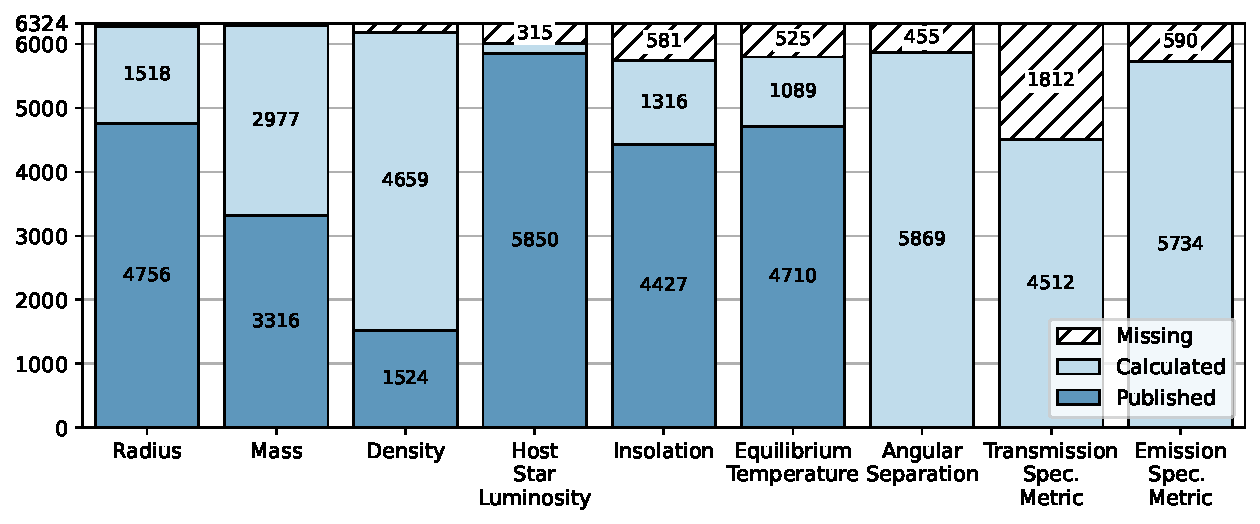
\includegraphics[width=\linewidth]{figures/nea_parameter_provenance.pdf}
    \caption{Provenance of \texttt{pscomppars} values (out of \num{6324} confirmed planets in
total) for the nine columns in which NEA reports ``Calculated Value'' entries.
All other columns are devoid of computations. Each bar splits the catalog into
entries with a directly published measurement, entries calculated by the
archive, and entries for which the parameter is missing entirely \cite{NasaExoplanetArchive}.
}
    \label{fig:calculated_columns}
\end{figure}

Exo-MerCat (\textit{Exoplanet Merged Catalog}) is a piece of Python software designed to generate a catalog of exoplanets, where data is merged from the most prominent exoplanetary catalogs (NASA Exoplanet Archive \cite{NasaExoplanetArchive}, Exoplanets Encyclopaedia \cite{ExtrasolarPlanetsEncyclopaedia}, Open Exoplanet Catalogue \cite{OpenExoplanetCatalogue}, the TESS Objects of Interest Catalog \cite{TessObjectsOfInterestCatalog} and the EPIC/K2 Objects of Interest Catalog \cite{K2CandidatesAndConfirmedPlanets}). Exo-MerCat removes computed quantities from catalogs and chooses the most precise quantities from the catalog list. 
It creates a large table with homogenized column names and units. Exo-MerCat also saves the catalogs in which it finds the planets, since a given planet may appear in multiple catalogs. A breakdown of the sources in the form of a UpSet-plot can be seen in \cref{fig:upset}. 

One important caveat that applies to both the NEA table and Exo-MerCat is that parameters for a given planet may not be self-consistent, as such planet-specific computations should be treated with caution \cite{NasaExoplanetArchive, Alei_2020, Alei_2025}. We will explicitly calculate some missing parameters. Thus all results involving some calculation, which we always clearly mark, should be treated with caution.


\begin{figure}[H]
    \centering
    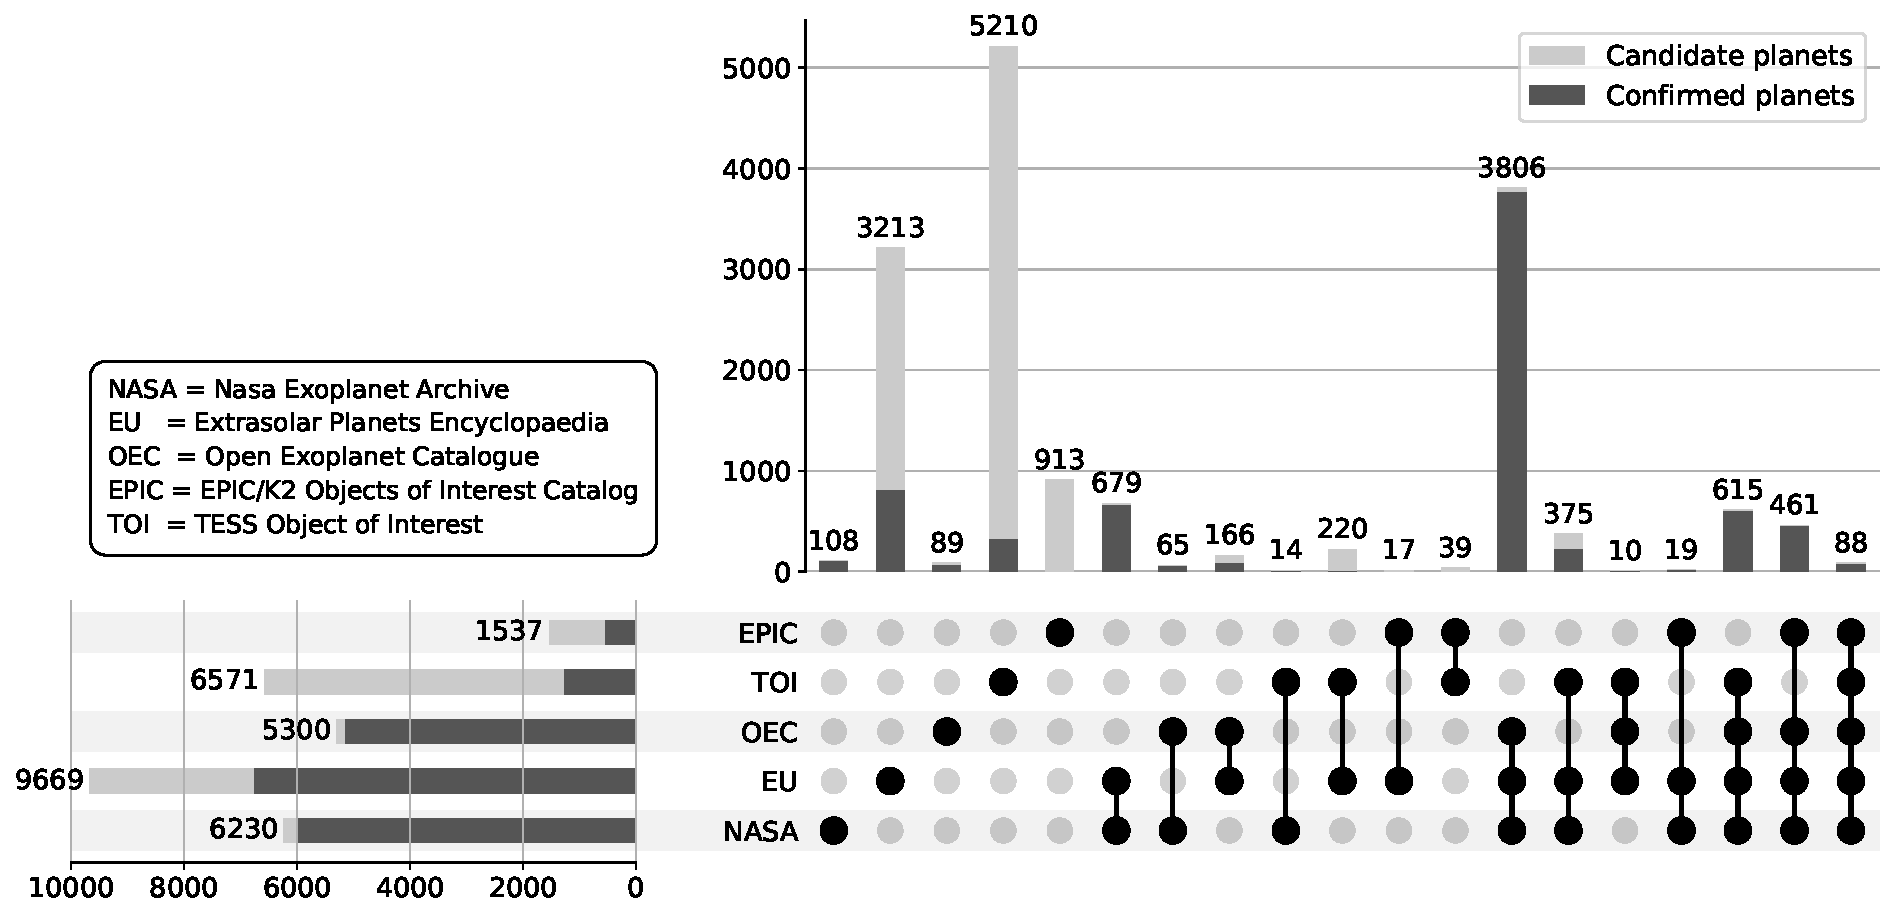
\includegraphics[width=\linewidth]{figures/exomercat_catalog_overlap_upset.pdf}
    \caption{UpSet plot showing the overlap and distribution of exoplanets across the source catalogs of Exo-MerCat. The horizontal stacked bar chart on the  left indicates the total count of planets in each catalog, while the vertical stacked bar chart at the top shows the size of the intersections of catalogs. Intersections with less than ten elements are omitted for brevity. A black dot on the line of a certain catalog means all planets in the vertical segment representing an intersection appear in that catalog. The bars are color-coded by planet status to differentiate between confirmed planets and candidate planets.}
    \label{fig:upset}
\end{figure}






\subsection{Conventions}
A candidate exoplanet is a suspected planetary signal that requires further validation to rule out astrophysical false positives. Conversely, a confirmed exoplanet is a candidate whose planetary nature has been independently detected using complementary observational techniques, establishing a high degree of physical certainty. Some catalogs such as NASA Exoplanet Archive and Open Exoplanet Encyclopedia carry only confirmed planets\footnote{The entries shown as candidate planets are ones that Exo-MerCat has flagged as "Controversial" since another catalog doesn't see them as confirmed}, while others such TESS object of Interest Catalog and EPIC/K2 Candidate Planet Catalog carry both types. Exo-MerCat has its own internal rules on how to assign a planet status and this work, we accept their treatment of the matter and treat both kind of planets, but always distinguish between them.

Of particular interest are potentially habitable planets which are commonly defined as the planets able to host liquid water. We will be working with the conventions of the LIFE collaboration, defining habitable planets by being temperate in the sense that the insolation flux lies in the range of $\qtyrange{0.35}{1.7}{\Searth}$ \cite{Kopparapu_2014} and that they may be rocky, which we define by the planetary radius being in the range of $\qtyrange{0.5}{1.5}{\Rearth}$ \cite{life4} \label{lab:hz_def}.












\newpage
\section{Methods}


\subsection{Python Package}
The crossmatching and enrichment pipeline described in this work is implemented as an open-source Python package, available at \sloppy{\url{https://github.com/JoshuaDreier/ExoplanetCrossmatcher}}. It makes extensive use of the package \texttt{astropy} \cite{astropy:2013, astropy:2018, astropy:2022}, using \texttt{astropy.table.Table} as the primary data structure throughout, so  that all intermediate and final outputs are directly compatible with the broader astronomical Python ecosystem. Astropy's connection to \texttt{pandas} \cite{pandas} and \texttt{numpy} \cite{numpy} was leveraged at multiple points in the code. Remote catalog access is handled via the Table Access Protocol (TAP) through \texttt{pyvo} (package associated with Astropy), with queries issued to the NASA Exoplanet Archive and SIMBAD endpoints. The package was developed and tested under Python~3.14.                      
The package was written in a catalog-agnostic way, such that the planetary catalog as well as the stellar catalog are parameters of the code and can easily be changed. The same is true for the service supplying alternate identifiers. The NASA Exoplanet Archive and Exo-MerCat catalog were implemented and specifically developed for this project. As a source for alternate identifiers SIMBAD and Exo-MerCat were added. For instructions and details on the crossmatching and enrichment code, refer to the code documentation contained in the repository.

Using $\texttt{pytest}$ \cite{pytest}, an end-to-end test suite uses the written code to match a set of known exoplanet host stars against all supported catalog and identifier-supplier combinations, asserting both that all expected planets are recovered and that no false positives are introduced. The identifier  normalization rules described in \cref{sec:id_matching} were each developed by inspecting coordinate-matched planets that were not recovered by  identifier matching, and were only retained after confirming they introduced no spurious matches in the test set.
Furthermore, functional tests and unit tests were written alongside the crossmatching and enrichment code, double-checking most non-trivial functions for possible bugs, ensuring that human-made coding errors are mitigated before `live-runs` yielding the actual data for this report.

\subsection{Identifier-based crossmatching}
\label{sec:id_matching}

Matching stellar catalogs by name is the most precise crossmatching strategy available: when the same physical object appears in both the input survey and the planet catalog under a common identifier, no position measurement is required and no false positives from chance alignments can arise.
The pipeline therefore prioritizes identifier-based matches over coordinate-based ones.

A key challenge in name-based catalog matching is that astronomical objects carry many designations: TIC numbers, HD/HIP/Gaia identifiers, common names, etc. none of which are guaranteed to appear in every catalog. To overcome this, the crossmatching queries the SIMBAD astronomical database \cite{Simbad} for every star in the input catalog, retrieving the full set of known identifiers for each object.
For out input catalog, this produces a table of roughly 300\,000 (input-star, alias) pairs. Exo-MerCat already provides an "alternate-identifiers" column, in which case the identifiers are taken from there and the SIMBAD querry is omitted (Note that Exo-MerCat uses SIMBAD internally). 

SIMBAD Identifier strings are not always directly compatible with how the stars are named in planetary catalogs. Therefore a few additional alternative identifiers are computed to increase the number of correct matches. Here follows a list of the additional alternate identifiers added for each identifier of a certain type. This was done by manually looking of the sample of coordinate-matched but not ID-matched planets and inspecting their alternate identifiers. This way most naming inconsistencies in the catalog dataset became apparent and were adjusted for:
\begin{enumerate}
    \item White-Space is normalized for all identifiers, some services store double spaces between catalog names and numbers (e.g. SIMBAD's \ \texttt{Ross~~128})
    \item Object-type prefixes (\texttt{*} or \texttt{**}) are stripped (e.g.\ \texttt{* alf~Cen} $\to$ \texttt{alf~Cen}), 
    \item The \texttt{NAME} prefix is removed (e.g.\ \texttt{NAME Proxima~Cen} $\to$ \texttt{Proxima~Cen})
    \item Possessive suffixes are dropped (e.g.\ \texttt{Barnard's} $\to$ \texttt{Barnard}).
\end{enumerate}

If the IDs are taken from Exo-MerCat other normalization rules are applied 
\begin{enumerate}
    \item White-space normalization
    \item capitalizing the \texttt{Gaia} prefix to \texttt{GAIA}
    \item TIC identifiers (\texttt{TIC-}\textit{N}) to the space-separated form (\texttt{TIC~}\textit{N}) 
\end{enumerate} 
 All of these extra rules were verified to not produce extra false positives by comparing the entirety of the matched planets with a rule added to the same sample matched without that rule and confirming that the differently matched planets are close-enough in coordinates or in some cases manually inspecting them using SIMBAD to see if they are the same object.
 

In \cref{sec:results} (Results) it is made clear that this is the most important matching method by number of matched planets.

Identifier crossmatching can also be used to detect and delete duplicates appearing, for example after merging parts of LIFEcat with HPIC.

\subsection{Coordinate-based matching}
Coordinate-based crossmatching serves as a complementary fallback for planets whose host star name could not be matched by any known identifier. For each row in the planet catalog, the closest star in the input catalog is found by angular distance, and the pair is accepted if that distance falls 
within a certain search radius $r$.

This is deliberately asymmetric. The search runs over the planet catalog, not the input catalog. This naturally handles multi-planet systems, such that all planets sharing a host star are each matched independently to the same input star. 

The search radius is not the same for all planets. For catalog rows where the proper motion $\mu$ and its upper uncertainty $\sigma^+_\mu$ are known, the radius grows with the  expected positional drift between the planet catalog's coordinate epoch and the input catalog's epoch:
\begin{equation}
    r = (\mu + \sigma_{\mu}^+)\,|\Delta t_i| + r_0
\end{equation}
where $r_0 = 10''$ is the base tolerance and $\Delta t_i$ is the epoch difference in years.  
Since proper motion is typically assumed to be approximately uniform rectilinear motion \cite{GaiaEDR3Astrometry}, this formula describes an approximate maximum angular distance a star can have traveled in the time between the two epochs.
For rows where the proper motion or epoch is unknown, a conservative flat radius of $50''$ is used instead. These values are calibrated empirically in \cref{sec:coordinate_calibration}.
With the current implementation, proper motion needs to be present as a property of the host star on the planet catalog side. Thus, only crossmatching against the NASA Exoplanet Archive can make use of the proper-motion-sensitive coordinate crossmatching, as it carries the PM values for its host star, which all other catalog sources of Exo-MerCat and Exo-MerCat itself do not. In principle however, with significant code adjustments, the matching algorithm could be written to take into account the proper motion on the stellar catalog side instead. As shown in the results section, the difference in accuracy is not large for our sample, because of the sparse density of exoplanet catalog entries at the time of writing.


The adopted tolerances are large compared to the $1''$ used in Exo-MerCat v2.1.0 (Exo-MerCat v1.0.0 used search radii of up to 36'')\cite{Alei_2025}. This is deliberate, as the appropriate value should be determined by the positional uncertainties of both catalogs, the epoch difference between them, and the on-sky density of the searched catalog. Since NEA does not publish per-row positional uncertainties and its coordinates are heterogeneously sourced (cf. \cref{sec:coordinate_calibration}), the uncertainty term is replaced by the fixed base tolerance $10''$, chosen generously enough to absorb the worst coordinate entries. 
Such generous radii are only admissible because the searched catalog is sparse. HPICxLIFEcat contains roughly $10^4$ stars spread over the full sky, corresponding to a surface density of $\rho\approx 2\times10^{-8} \,\text{arcsec}^{-2}$. The probability of a chance alignment is therefore of order $\pi r^2 \cdot \rho \approx \num{2E-6}$ per planet row for the base tolerance and $\num{5E-5}$ for the $50''$ fallback, yielding an expectation value of $\sim 0.65$ false matches and luckily none are found in the empirical calibration (\cref{sec:coordinate_calibration}). 

\subsection{Post-matching data enrichment}

After crossmatching, many planet catalog rows are missing stellar or orbital parameters needed for candidate filtering or other uses. An enrichment step fills these gaps by merging values from additional catalog sources in a fixed priority order. The sources used here are, from highest to lowest priority: the input HPIC catalog, the NASA Exoplanet Archive composite parameters table, the Exoplanets Encyclopaedia, the K2 EPIC catalog, the TESS Objects of Interest catalog, and SIMBAD stellar parameters. The first source that provides a non-masked value for a given parameter is taken as the entry for that quantity. 

After sourcing, for still missing parameters, calculations are executed to give broad estimates for a subset of the sourced quantities. Each output parameter is accompanied by a provenance string that records which source or formula supplied the value.

The list of parameters that are sourced from catalogs are: planetary radius $r_p$, planetary mass $m$, projected planetary mass ($m \sin i $) planetary insolation flux $S$, planetary equilibrium temperature $T_\text{eq}$, orbital semi-major axis $a$, orbital period $P$, host star spectral type (MK system), host star radius $R_*$, host star mass $M_*$, host star effective temperature $T_\text{eff}$, host star surface gravity $\log g_*$, host star metallicity $\ce{Fe/H}$, host star luminosity $L_*$, host system distance $d$ and the magnitude brightness of the host star system in the Visual and Kepler bands.

For parameters that remain missing after source merging, a cascade of physically motivated fallback derivations is applied. Treating the variables as uncorrelated, gaussian error propagation is applied where possible to retain a sense of accuracy after the quantities have been computed. The derivations execute in the order listed below, each running only when its inputs are available and the target quantity is still missing.
\begin{itemize}
    \item Host star effective temperature: Inferred from spectral type, interpolating between anchors from \textcite{PecautMamajek2013} and \textcite{Martins2005}, or via Stefan Boltzmann relation $T_\text{eff}^4\propto \dfrac{L_*}{R_*²}$
    \item Host star Luminosity: $L_\star \propto  R_\star^2 T_\mathrm{eff}^4$ (Stefan-Boltzmann)
    \item Host star radius: The following options are tried, stopping at the first success, (methods decreasing in precision):
    \begin{itemize}
        \item $R_*^2 \propto M_* / g_*$
        \item $R_*^2 \propto \dfrac{L_* }{T_\text{eff}^4}$  (Stefan Boltzmann)
        \item \textcite{Mann2015} empirical relation dependent on the absolute K-band magnitude $M_K$, which is calculated from the K-band magnitude and distance (only applicable for $T_\text{eff} < \qty{4200}{\kelvin}$ and $M_K \in[4.0, 10.5]$). Then $R_*$ follows from a second degree polynomial in $M_K$ with a prefactor dependent on $\ce{Fe/H}$.
        \item \textcite{Torres2010} empirical relation applicable ($T_\text{eff}$ from $\qtyrange{3900}{8500}{\kelvin}$), giving $\log R_*$ as a third degree polynomial in $\log T_\text{eff}, \log g, \ce{Fe/H}$.
        \item \textcite{Mann2015} empirical relation for late K and M dwarfs ($T_\text{eff} < \qty{4000}{\kelvin}$), giving $R_*$ as a third degree polynomial in $T_\text{eff}$
        \item \textcite{Boyajian_2012one,Boyajian_2012two, Boyajian_2013} zero-age main-sequence relation between $R_*$ and $T_\text{eff}$, expressed as a piece-wise power law clamped at $\qty{0.05}{\Rsun}$
    \end{itemize}
    \item Host star mass: $M_* \propto R_*^2 g_*$
    \item Orbital semi-major axis:  $a^3  \propto M_* P^2 $ (Kepler's third law)
    \item Planet Equilibrium Temperature: $T_\text{eq} ^4\propto S$, (taking earth's eq. temperature with a Bond albedo of $A_B  = 0.3$ as a reference.)
    \item Planet insolation: $S \propto L/a^2$ or via reversing equilibrium temperature formula above

\end{itemize}                  
Further calculation details can be found in the code documentation. A breakdown of the number of times each computation was employed for the dataset we are working with can be found in \cref{fig:enrichment_mermaid} in the appendix \cref{appdx:enrichment}. The enrichment leads to $\sim50$\% more more planet entries in Exo-MerCat having insolation values that we can work with to characterize the population in \cref{sec:results}. 

For radial-velocity planets with no directly measured radius, radius bounds are estimated from $m\sin i$ using the Chen \& Kipping \citeyear{ChenKipping2017} probabilistic mass-radius relation. The lower bound is $R_\mathrm{CK}(m\sin i)$ and the upper bound is $R_\mathrm{CK}(m\sin i 
/ \sin i_\mathrm{min})$ with a default $\sin i_\mathrm{min} = 0.3$, based on averaged posterior-distribution estimates from \textcite{HoTurner2011}, giving a broad interval that keeps such planets visible in candidate-filtering workflows without asserting a definite radius. Similarly planet with known masses but unknown radius are given radius estimates with the same relation. This is the case for around 10\% of all Exo-MerCat planets.

These enriched parameters are then used to classify planets as potentially rocky ($r_p$ from $\qtyrange{0.5}{1.5}{\Rearth}$) and potentially temperate ($S$ from $\qtyrange{0.35}{1.7}{\Searth}$), described further in Section~\ref{sec:results}, in accordance with the definition given in \cref{lab:hz_def}.


\subsection{Exo-MerCat}
At the time of writing, the Exo-MerCat \cite{Alei_2020, Alei_2025} TAP service is not actively updated. To guarantee up-to-date results, a local installation was used. The results in this report are based on Exo-MerCat v2.1.0 run on July 13, 2026, using the source catalogs most recent versions at that time.

\newpage
\section{Results \& Discussion}\label{sec:results}
\subsection{Matching}
\subsection{Coordinate Matching}
\label{sec:coordinate_calibration}

\begin{wrapfigure}[39]{r}{0.5\textwidth}
    \vspace{-3cm}
    \centering
    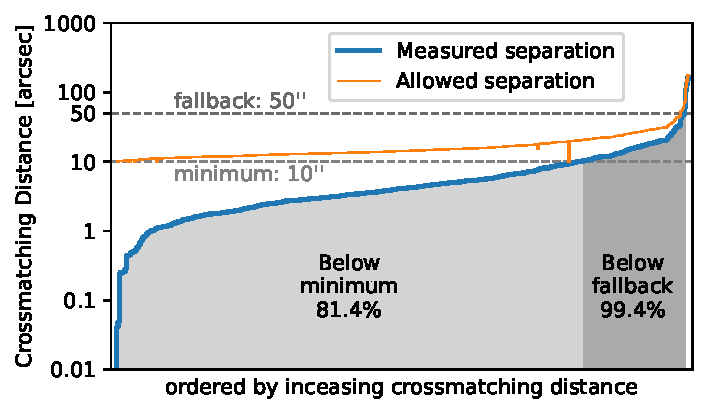
\includegraphics[width=\linewidth]{figures/nea_coordinate_calibration.pdf}
    \caption{Calibration of coordinate crossmatching for NEA using SIMBAD IDs to crossmatch with HPICxLIFEcat. The separations between matched HPICxLIFEcat input stars and NEA catalog positions are plotted in increasing order and the algorithm’s 10'' minimum matching tolerance and 50'' fallback threshold overlaid to illustrate how the observed IDs fall within the adopted angular acceptance. The remaining 0.6\% above the fallback threshold are also coordinate matched due to the proper-motion-sensitive search radius.}
    \label{fig:nea_coord_cal}
    \vspace{0.5cm}
    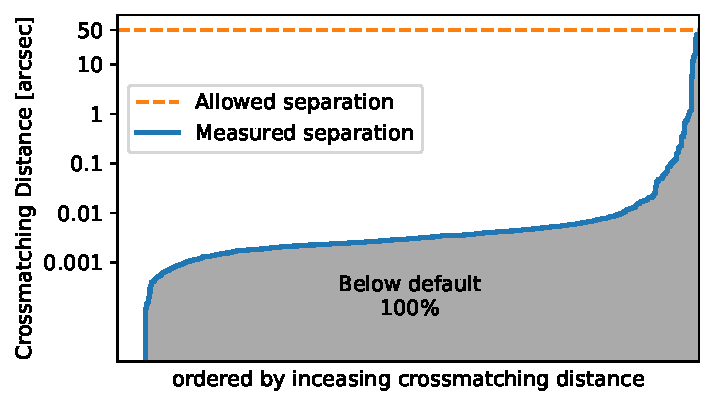
\includegraphics[width=1\linewidth]{figures/emc_coordinate_calibration.pdf}
    \caption{Calibration of coordinate crossmatching for EMC using ID crossmatches showing the measured angular separations for matched HPICxLIFEcat stars with the 50'' matching tolerance annotated to demonstrate that all ID-based matches remain within the adopted acceptance radius}
    \label{fig:emc_coord_cal}
    \vspace{0.5cm}
    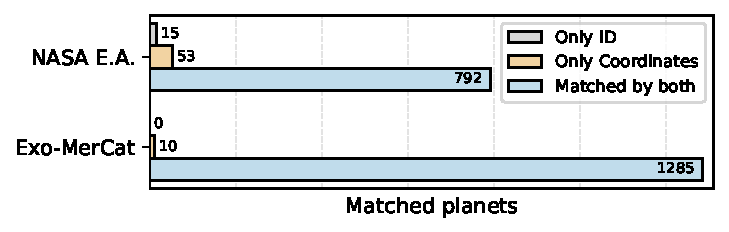
\includegraphics[width=\linewidth]{figures/crossmatch_yield.pdf}
    \caption{Yield of matched planets for the NASA Exoplanet Archive and Exo-MerCat catalogs, categorized by which methods the match was established.}
    \label{fig:yield}
\end{wrapfigure}



The NASA exoplanet archive (shortened here to NEA) is by far the most cited exoplanet catalog and thus deserves special attention among the input sources. NEA's coordinates are assembled from many different sources and the coordinate epoch can be read or estimated from the source they list for the entry. As can be seen in \cref{fig:nea_coord_cal}, using the proper-motion-aware formula on a set of ID-matched stars, we achieve a matching accuracy of 100\%. Neglecting the proper motion correction, we see that 50'' is a reasonable threshold for matching when that option is not available. By comparing the distances to the next-nearest neighbors in the HPICxLIFEcat catalog, we also find that 50'' leads to no predicted false positives.




Exo-MerCat does not carry columns for proper motion, thus only a "default" search radius can be applied. Despite this, as is observed in \cref{fig:emc_coord_cal}, the average crossmatching distance between HPICxLIFEcat and Exo-MerCat is generally around two orders of magnitude smaller than the average crossmatching distance between HPICxLIFEcat and NEA (c.f. \cref{fig:nea_coord_cal}). This relates to the fact that Exo-MerCat takes its coordinates from SIMBAD, which for HPICxLIFEcat is also the primary data source. In opposition, NEA carries its own heterogeneously sourced coordinate entries, many of which do not even carry the same epochs and sometimes reach back to the mid 20th century. As before, the likelihood of false positives stays low due to the low density across the sky. 




\subsection{Combined Matching}
As shown in \cref{fig:yield}, coordinate-only matching proves to be the edge case, as matching with NEA and Exo-MerCat primarily results in matches based on linked identifiers. As expected, Exo-MerCat matches are almost a superset of the NEA matches. The only exceptions are high-mass directly imaged planets that were removed by Exo-MerCat's BD-removal step. The lower count of only-coordinate matches can primarily be explained by Exo-MerCat's internal alternate ID handling, which covers more cases than the one implemented for SIMBAD in this project.

\subsection{Population Analysis}
Exo-MerCat assembles the largest published list of exoplanets, and is thus very useful in gaining a sense of the broader known planet population. In \cref{fig:pop_distr} we can see certain features of the diagram correspond to specific parts of the exoplanet population (Note that part of the data was taken from post-Exo-MerCat enrichment computations, a version without can be found in \cref{fig:pop_distr_nocomp} in appendix \cref{appddx:nocomp}): For example the "bulge" on the top right (high insolation, high radius) represents the hot jupiter type planets. The long thin strand pointing downwards on the right half of the plot are wide-separation planets observed via direct imaging. The bunching around $\qty{E1}{\Rearth}$ is likely a consequence of the \textcite{ChenKipping2017} power law's local maximum around that value, which NEA uses internally to compute radii from masses when their missing \cite{NasaExoplanetArchive}. 

\begin{figure}[ht]
    \centering
    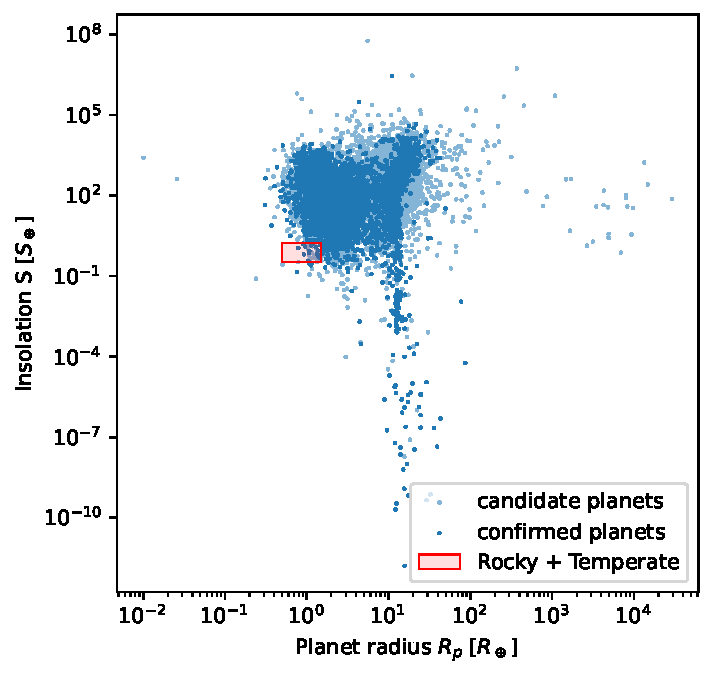
\includegraphics[width=0.72\textwidth]{figures/radius_insolation_distribution.pdf}
    \caption{Distribution of the enriched Exo-MerCat exoplanet population in terms of planet-radius insolation (contains parameter computations). Confirmed planets are drawn in the darker shade and unconfirmed candidates in the lighter shade. The red rectangle marks the rocky-and-temperate selection region adopted in this work, spanning a radius of $0.5$--$1.5\,R_\oplus$ and an incident stellar flux of $0.35$--$1.7\,S_\oplus$.}
    \label{fig:pop_distr}
\end{figure}

We can compare the overall distribution with just the distribution of planets matched by HPICxLIFEcat, here done in heatmap form to better assess how many planets share similar parameters, presented in \cref{fig:pop_heatmap} (and a decomposition into the spectral categories of the same heatmap in appendix \cref{appdx:spectral_category} \cref{fig:pop_heatmap_spectral}). Note that the feature of hot jupiters is absent in the left side since low-mass stars are known to rarely host hot jupiters \cite{Ganetal2023}. Because very-low-luminosity stats are highly abundant in our solar neighborhood, they dominate the HPICxLIFEcat stellar population and host nearly all of these planets. We are not excluding any planets from being classified as temperate and rocky by undershooting the $0.5\Rearth$ boundary, which is likely due to observational biases against low-mass/radius and comparatively long-period planets \cite{Guyon2017}.


\begin{figure}[ht]
    \centering
    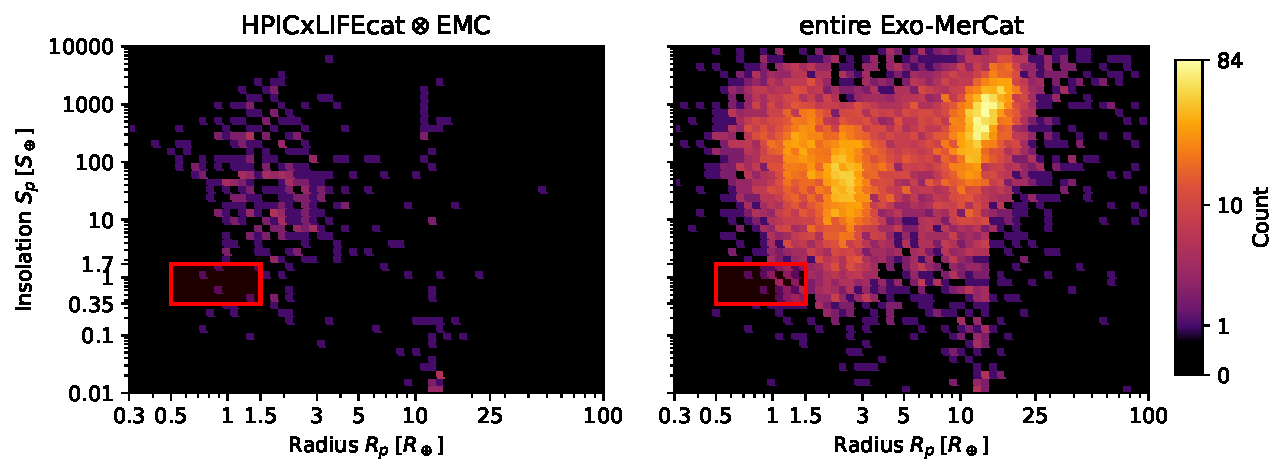
\includegraphics[width=\textwidth]{figures/radius_insolation_heatmap.pdf}
    \caption{Two-dimensional number density heatmap of the known exoplanet population w.r.t planet-radius and insolation comparing the distributions in Exo-MerCat and Exo-MerCat matched to HPICxLIFEcat. The red rectangle marks the same rocky-and-temperate selection region as in \cref{fig:pop_distr}, spanning $0.5$--$1.5\,R_\oplus$ and $0.35$--$1.7\,S_\oplus$. A breakdown of the same distribution by host spectral category is given in \cref{fig:pop_heatmap_spectral}.}
    \label{fig:pop_heatmap}
\end{figure}

Particularly interesting to the LIFE mission is the population of rocky habitable zone planets. We categorize stars into three categories based on their spectral type: Sun-like (F0V-K5V), Low-luminosity (K6V-M2V), and Very-low-luminosity (M3V-M9V). All left over spectral types and non-main-sequence stars are grouped as "Other".  Furthermore, working with the definition \cref{lab:hz_def} we differentiate between two kinds planets can be classified as rocky and temperate. The first one is "Confirmed", when its published values lie within our definition. "Uncertain" means the planet might be rocky and temperate in the sense that it is either a candidate planet meeting the requirements or a planet whose measurement error in the relevant quantities makes the allowed parameter range overlap with our definition of habitable. The full list of rocky, temperate planet candidates underlying \cref{fig:rocky_temp_yield} is given in \cref{appdx:rocky_temp_tables}: \cref{tab:rocky_temp_table} for the distance-limited HPIC$\times$LIFEcat crossmatched sample and \cref{tab:rocky_temp_table_full} for the entire Exo-MerCat catalog.

\begin{figure}[H]
    \centering
    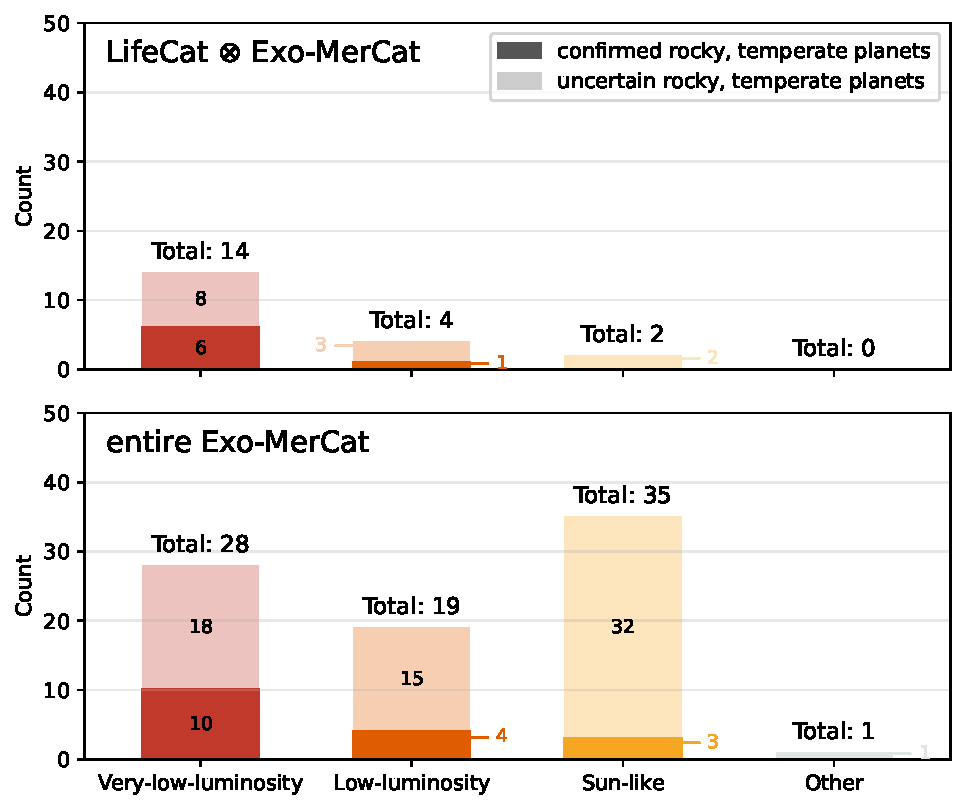
\includegraphics[width=0.9\textwidth]{figures/rocky_temperate_yield.pdf}
    \caption{Yield of rocky, temperate planet candidates by host-star spectral category, using the same selection region as \cref{fig:pop_distr} and \cref{fig:pop_heatmap} (radius $0.5$--$1.5\,R_\oplus$, insolation $0.35$--$1.7\,S_\oplus$). A planet is counted as confirmed (dark shading) if its central-value radius and insolation both fall inside the box and it is a confirmed planet, and as uncertain if the box is met only within the uncertainty of the radius/insolation uncertainty interval, or if the central values fall inside the box but the planet is not confirmed. The top panel shows the distance-limited HPIC$\times$LIFEcat sample crossmatched with Exo-MerCat (20 candidates in total), the bottom panel the entire Exo-MerCat catalog (83 candidates in total). The full list of candidates is given in Appendix \cref{appdx:rocky_temp_tables}.}
    \label{fig:rocky_temp_yield}
\end{figure}


\subsection{Outlook}
This project stands as a tool to quickly and reliably match known exoplanets to any stellar catalog, which can be used in the future for yield estimates similar to how a simulated exoplanetary catalog was employed by \textcite{life4}. Furthermore, this work may be used for studies similar to \citetitle{Life10} by \textcite{Life10} by providing a quick and repeatable way of selecting potentially habitable planets to then study on a case by case basis.

On the enrichment side, by comparing and potentially adopting some of \citetitle{Bohl_2026} by \textcite{Bohl_2026} methods, better enrichment pathways can be exploited to further increase the number of paper-sourced parameters and use more accurate methods for inferring missing parameters to get a better sense of the broader exoplanet population.


\section{Conclusion}
In this work we presented an open-source, catalog-agnostic Python package that crossmatches a stellar catalog against a planetary catalog and enriches the matched planets with stellar and planetary parameters. Applied to HPICxLIFEcat, the pipeline was run against both the NASA Exoplanet Archive and Exo-MerCat, prioritizing identifier-based matching, using alternate identifiers from SIMBAD and Exo-MerCat, over a proper-motion-aware coordinate-based fallback.

Identifier-based matching proved to be the dominant matching method by number of matched planets, with coordinate-only matches remaining the edge case. Calibrating the coordinate thresholds on ID-matched stars showed that the proper-motion-aware search radius with a base tolerance of $10''$ recovers all matches against NEA, and that the flat $50''$ fallback radius is sufficient when proper motion is unavailable; in both cases the sparse on-sky density of exoplanet hosts leads to no predicted false positives. The Exo-MerCat matches form a near superset of the NEA matches.

After enrichment from a priority-ordered set of catalog sources and physically motivated fallback derivations, the combined catalog yields 20 rocky, temperate planet candidates around HPICxLIFEcat stars (7 confirmed and 13 uncertain), out of 83 across the entire Exo-MerCat catalog. These planets are hosted almost exclusively by M dwarfs, reflecting the abundance of cool, low-mass stars in the immediate solar neighborhood that dominates the LIFE target list. This list provides a set of already-known targets relevant to LIFE's search phase, and, owing to the catalog-agnostic design of the package, can be regenerated quickly as the stellar target-selection catalog and the planetary catalogs evolve.


\newpage
\section{Acknowledgments}
The author thanks  his advisor Lia Sartori for their guidance, continuous support and prompt responses, as well as his friends, Pascal D'Andrea and Johanna Kroker for proofreading and helpful discussions.

The author acknowledges using generative AI (Claude Code, Google Gemini) for the purpose of aiding in formatting the \LaTeX-document, \texttt{matplotlib.pyplot} plots and as a search tool for finding relevant literature. The python package was extensively tested with AI-written testcases, the relevance and truthfulness of which was always verified by the author. The author notes that no AI tools were used in the textual writing of the document (with the exception of checking for typos, and converting the summary into an abstract) and in the core logic of the code, excluding the aforementioned test cases.
\vspace{3cm}
\printbibliography

\appendix   

 \section{Enrichment Pipeline}
  \label{appdx:enrichment}
 
 \begin{figure}[H]
     \centering
     \vspace{-0.5cm}
     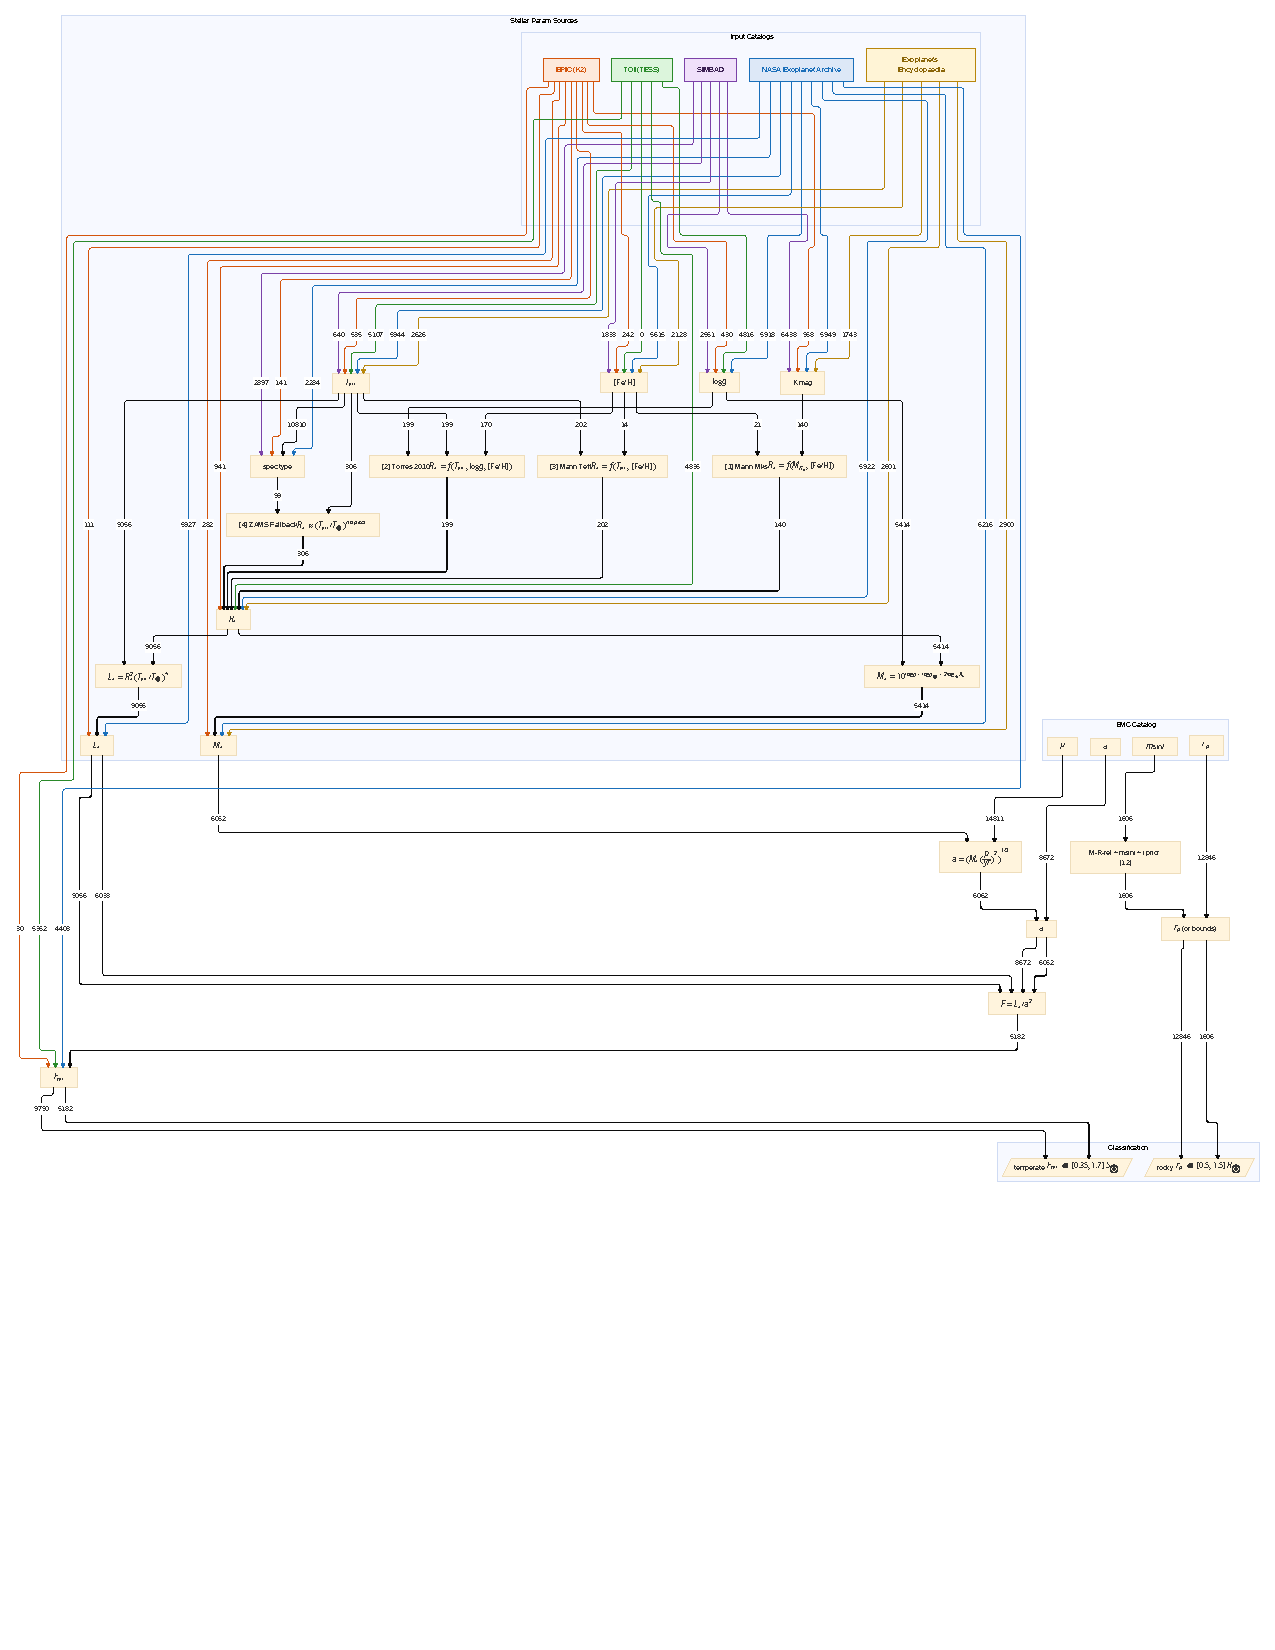
\includegraphics[width=0.9\linewidth]{figures/enrichment_pipeline_flowchart.pdf}
     \vspace{-4cm}
     \caption{The flowchart illustrates the priority-ordered data retrieval hierarchy from input sources and the subsequent empirical or  physical derivation pathways used to determine stellar parameters and orbital/planetary quantities. Solid arrows represent directly retrieved catalog values, while dashed arrows denote computed properties, with labels indicating the exact number of planet-rows processed through each transition.}
     \label{fig:enrichment_mermaid}
 \end{figure}


\section{Planet distribution without parameter computations}
\label{appddx:nocomp}
\begin{figure}[H]
    \centering
    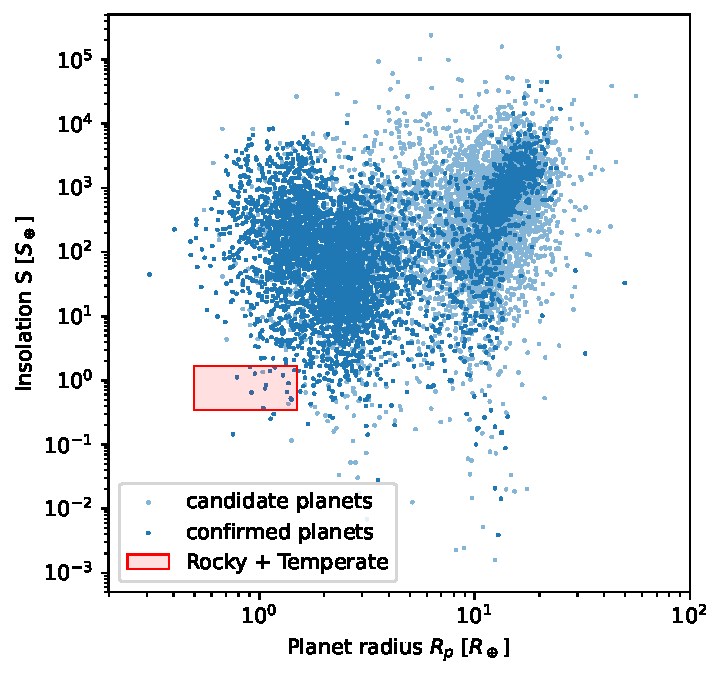
\includegraphics[width=0.72\textwidth]{figures/radius_insolation_distribution_uncomputed.pdf}
    \caption{Distribution of the enriched Exo-MerCat exoplanet population in terms of planet-radius insolation (contains no parameter computations). Confirmed planets are drawn in the darker shade and unconfirmed candidates in the lighter shade. The red rectangle marks the rocky-and-temperate selection region adopted in this work, spanning a radius of $0.5$--$1.5\,R_\oplus$ and an incident stellar flux of $0.35$--$1.7\,S_\oplus$.}
    \label{fig:pop_distr_nocomp}
\end{figure}

\section{Population by Host Spectral Category}
\label{appdx:spectral_category}

\Cref{fig:pop_heatmap_spectral} splits the planet-radius--insolation density of \cref{fig:pop_heatmap} by the spectral category assigned to the host star by the enrichment pipeline. As expected from the broader field, Sun-like hosts dominate the overall Exo-MerCat population. In the distance-limited HPICxLIFEcat crossmatch, however, the low- and very-low-luminosity categories carry a markedly larger share of the sample ($\sim$35\% of the crossmatched planets versus $\sim$12\% of the full catalog), reflecting the abundance of cool, low-mass stars in the immediate solar neighborhood that dominates the LIFE target list.

\begin{figure}[H]
    \centering
        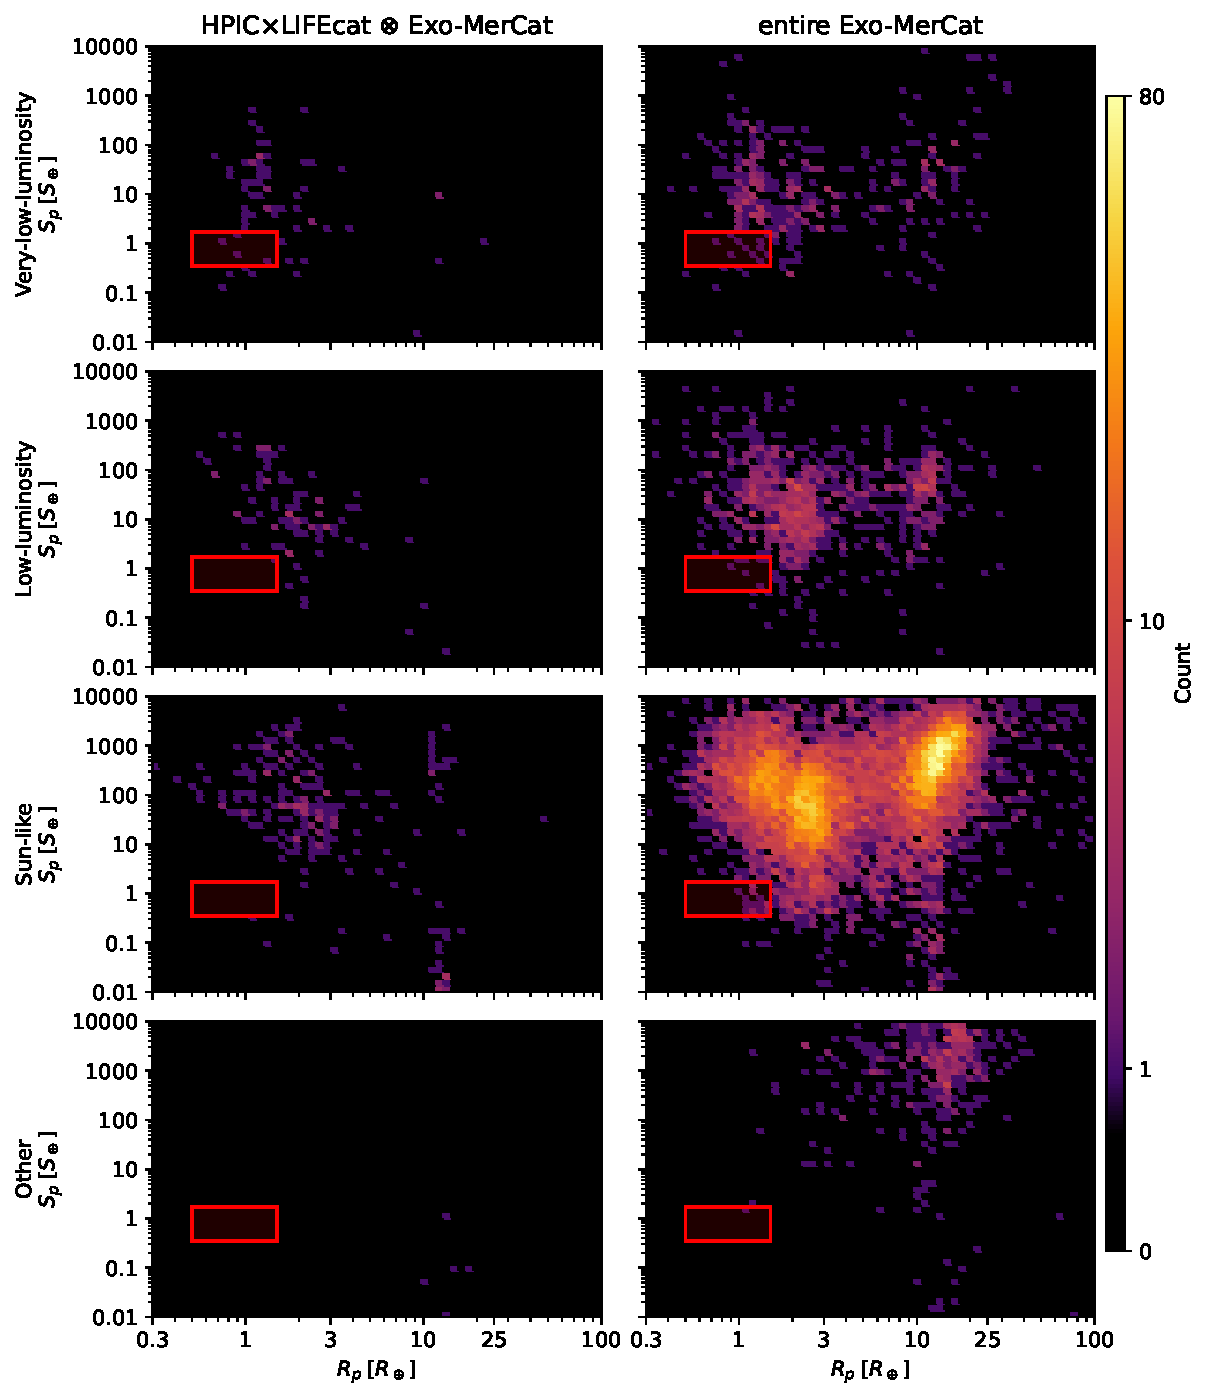
\includegraphics[width=0.9\linewidth]{figures/radius_insolation_heatmap_by_spectral_category.pdf}
    \caption{Two-dimensional number density of the exoplanet population in the planet-radius--insolation plane (as in \cref{fig:pop_heatmap}), split by the spectral category of the host star. The four rows correspond to the host categories assigned by the enrichment pipeline (Very-low-luminosity, Low-luminosity, Sun-like, and Other); the left column is the distance-limited HPIC$\times$LIFEcat sample crossmatched with Exo-MerCat and the right column the entire Exo-MerCat catalog. Both axes are logarithmic and the color encodes the number of planets per bin on a logarithmic scale, shared across all panels. The red rectangle marks the rocky-and-temperate selection region ($0.5$--$1.5\,R_\oplus$, $0.35$--$1.7\,S_\oplus$). Planet radii and insolations are those provided by the enrichment pipeline.}
    \label{fig:pop_heatmap_spectral}
\end{figure}

\section{Rocky, Temperate Planet Candidate Tables}
\label{appdx:rocky_temp_tables}

\Cref{tab:rocky_temp_table} lists the rocky, temperate planet candidates in the distance-limited HPIC$\times$LIFEcat sample crossmatched with Exo-MerCat (the same population as the top panel of \cref{fig:rocky_temp_yield}); \cref{tab:rocky_temp_table_full} lists the same selection applied to the entire enriched Exo-MerCat catalog (the bottom panel of \cref{fig:rocky_temp_yield}). 

\begin{landscape}
\centering
\input{figures/rocky_temperate_candidates_table.tex}
\end{landscape}

\begin{landscape}
\centering
\begin{longtblr}[
  caption = {Rocky, temperate planet candidates in Exo-MerCat (see \cref{fig:rocky_temp_yield})},
  label = {tab:rocky_temp_table_full},
]{colspec = {Q[l,wd=3.5cm] l l l l Q[l,wd=3cm] c}, font=\footnotesize, rowsep=1pt, row{1} = {font=\bfseries\footnotesize}, rowhead=1}
\hline\hline
Planet & Insolation Flux [\si{\Searth}] & Radius [\si{\Rearth}] & Mass [\si{\Mearth}] & Distance [\si{\parsec}] & Semi-major Axis [\si{\astronomicalunit}] & Spectral Type \\
\hline
\SetCell[c=7]{c}{\textbf{Confirmed}} \\
\hline
L 372-58 c & \num{1.40(20)} & \num{1.194(47)}\textsuperscript{c} & \num{1.81(13:11)} & \num{3.67278(89:90)} & \num{0.0350(10)} & M5.5 \\
L 372-58 d & \num{0.60(10)} & \num{1.149(76)}\textsuperscript{c} & \num{1.67(17:21)} & \num{3.67278(89:90)} & \num{0.0540(10)} & M5.5 \\
G 32-5 b & \num{1.62(13:11)} & \num{0.904(37:34)} & \num{0.71(12)} & \num{12.210(13)} & \num{0.06700(50:60)} & M3.0 \\
TRAPPIST-1 d & \num{1.115(43)} & \num{0.7880(110:100)} & \num{0.388(12)} & \num{12.430(19)} & \num{0.0223} & M8.0 \\
TRAPPIST-1 e & \num{0.646(25)} & \num{0.920(13:12)} & \num{0.692(22)} & \num{12.430(19)} & \num{0.0293} & M8.0 \\
TRAPPIST-1 f & \num{0.373(15:14)} & \num{1.045(13:12)} & \num{1.039(31)} & \num{12.430(19)} & \num{0.0385} & M8.0 \\
TOI-700 d & \num{0.850(90:100)} & \num{1.073(59:54)} & \num{2.42} & \num{31.127(21)} & \num{0.1633(27)} & M2.5 \\
TOI-700 e & \num{1.27(13:15)} & \num{0.953(89:75)} & \textemdash & \num{31.127(21)} & \num{0.1340(22)} & M2.5 \\
LP 890-9 c & \num{0.906(26)} & \num{1.367(55:39)} & \num{25(25)} & \num{32.430(70)} & \num{0.03984(22)} & M6 \\
K2-3 d & \num{1.44(14)} & \num{1.458(56:51)} & \num{2.20} & \num{44.07(11)} & \num{0.2014(34:33)} & M \\
LP 759-72 e & \num{1.20(20)} & \num{1.29(13)} & \textemdash & \num{66.43(20)} & \num{0.1060(90:130)} & \textemdash \\
Kepler-1649 A c & \num{0.750(32:302)} & \num{1.06(15:10)} & \textemdash & \num{92.19(55:54)} & \num{0.0649} & \textemdash \\
Kepler-1512 A b & \num{1.60(44:51)} & \num{1.180(70:110)} & \textemdash & \num{162.0(58:159)} & \num{0.13693(52)} & \textemdash \\
Kepler-438 b & \num{1.40(67:77)} & \num{1.12(16:17)} & \textemdash & \num{195.9(47)} & \num{0.166(51:42)} & \textemdash \\
Kepler-1229 A b & \num{0.524(54:50)} & \num{1.40(11:13)} & \num{2.54} & \num{265.5(34:33)} & \num{0.3006(69:91)} & M0 \\
Kepler-62 f & \num{0.500} & \num{1.412(67)} & \num{35.0} & \num{300.9(12)} & \num{0.7180(70)} & K2 \\
Kepler-442 b & \num{0.66(23:41)} & \num{1.35(18:11)} & \textemdash & \num{366.0(28:27)} & \num{0.409(209:60)} & \textemdash \\
\hline
\SetCell[c=7]{c}{\textbf{Uncertain}} \\
\hline
Proxima Centauri b & \num{0.641(65)} & \num{1.36(34)}\textsuperscript{c} & \num{1.055(55)}\textsuperscript{b} & \num{1.30119(34:35)} & \num{0.04848(29)} & M5.5 \\
Ross 128 b & \num{1.38} & \num{1.55(45)}\textsuperscript{c} & \num{1.40(21)}\textsuperscript{b} & \num{3.37454(80)} & \num{0.0496(17)} & M4 \\
Teegarden's Star b & \num{1.080(80)} & \num{1.42(37)}\textsuperscript{c} & \num{1.16(12:11)}\textsuperscript{b} & \num{3.8308(40)} & \num{0.02590(80:90)} & M7.0 \\
Teegarden's Star c & \num{0.350(20)} & \num{1.36(33)}\textsuperscript{c} & \num{1.05(14)}\textsuperscript{b} & \num{3.8308(40)} & \num{0.0443(14:15)} & M7.0 \\
G 158-27 b & \num{0.670(39)} & \num{1.37(34)}\textsuperscript{c} & \num{1.08(13)}\textsuperscript{b} & \num{4.8487(30)} & \num{0.0457(12)} & M5.5 \\
BD-17 588 A d & \num{1.00(45)}\textsuperscript{a} & \num{2.21(75)}\textsuperscript{c} & \num{2.721(75)}\textsuperscript{b} & \num{6.90} & \num{0.090(20)} & M3.5 \\
HD 156384 C e\textsuperscript{d} & \num{0.302(60)}\textsuperscript{a} & \num{2.20(75)}\textsuperscript{c} & \num{2.7(16:14)}\textsuperscript{b} & \num{7.2440(49:48)} & \num{0.213(20)} & M1.5 \\
HD 156384 C f\textsuperscript{d} & \num{0.56(13:11)}\textsuperscript{a} & \num{2.12(72)}\textsuperscript{c} & \num{2.5(13)}\textsuperscript{b} & \num{7.2440(49:48)} & \num{0.156(14:17)} & M1.5 \\
G 192-13 b & \num{0.910(90)} & \num{2.00(68)}\textsuperscript{c} & \num{2.30(40)}\textsuperscript{b} & \num{7.7227(48)} & \num{0.09673(80)} & M4 \\
Wolf 1069 b & \num{0.652(29:27)} & \num{1.48(40)}\textsuperscript{c} & \num{1.26(21)}\textsuperscript{b} & \num{9.5834(48)} & \num{0.0672(14)} & M5.0 \\
G 261-6 b & \num{1.80(12:11)} & \num{1.54(44)}\textsuperscript{c} & \num{1.37(23)}\textsuperscript{b} & \num{10.6267(63)} & \num{0.02971(87:93)} & M5.5 \\
L 291-115 b\textsuperscript{d} & \num{0.332(23)}\textsuperscript{a} & \num{0.79(17)} & \textemdash & \num{14.6058(61)} & \num{0.0699(14)}\textsuperscript{a} & M5 \\
HD 6660 .01\textsuperscript{d} & \num{1.39} & \num{2.24(92)} & \textemdash & \num{20.527(29)} & \num{1.87(14)}\textsuperscript{a} & K4 \\
TOI-4336 .01 & \num{1.69} & \num{2.05(76)} & \textemdash & \num{22.546(38)} & \num{0.0850(17)}\textsuperscript{a} & M3.5 \\
CD-34 1169 .01\textsuperscript{d} & \num{0.431} & \num{1.37(77)} & \textemdash & \num{25.143(30)} & \num{1.176(24)}\textsuperscript{a} & M \\
LP 873-20 b\textsuperscript{d} & \num{1.54}\textsuperscript{a} & \num{1.16(25)} & \textemdash & \num{26.075(22)} & \textemdash & \textemdash \\
2MASS J06034353-8127303 .01\textsuperscript{d} & \num{1.35} & \num{1.04(17)} & \textemdash & \num{26.741(63)} & \num{0.0258(13)}\textsuperscript{a} & \textemdash \\
G 125-49 b & \num{1.68(17:37)} & \num{1.65(22:20)} & \textemdash & \num{32.027(45)} & \num{0.05722(44)} & M3.5 \\
LSPM J1957+5658 .01\textsuperscript{d} & \num{0.382} & \num{1.81(66)} & \textemdash & \num{32.609(44)} & \textemdash & M4.0 \\
PM J13119+6550 d & \num{1.30(30:20)} & \num{1.70(58)}\textsuperscript{c} & \num{3.7(10:11)}\textsuperscript{b} & \num{36.012(30)} & \num{0.1513(24)} & M2 \\
MCC 189 .01\textsuperscript{d} & \num{0.406} & \num{1.74(84)} & \textemdash & \num{39.889(31)} & \num{1.51(16)}\textsuperscript{a} & M0 \\
LSPM J1902+7525 c & \num{1.84(17)} & \num{1.334(78)} & \num{7.40} & \num{41.918(50)} & \num{0.1370(60)} & M2.5 \\
TOI-715 b & \num{0.67(15:20)} & \num{1.550(64)} & \num{3.02} & \num{42.405(86:85)} & \num{0.0830(27)} & M4 \\
LP 425-186 .01\textsuperscript{d} & \num{35(32:39)}\textsuperscript{a} & \num{1.26(39:87)} & \textemdash & \num{42.89(18)} & \num{0.0117(23:40)}\textsuperscript{a} & \textemdash \\
HD 137010 b & \num{0.300(68:204)}\textsuperscript{a} & \num{1.060(61)} & \textemdash & \num{44.860(30)} & \num{0.88(30:10)} & K3.5 \\
2MASS J05021345+1442367 .01\textsuperscript{d} & \num{0.60(22)}\textsuperscript{a} & \num{1.233(116:94)} & \textemdash & \num{45.99(72)} & \num{0.05061(52)}\textsuperscript{a} & M4 \\
2MASS J05021345+1442367 .02\textsuperscript{d} & \num{0.268(98)}\textsuperscript{a} & \num{0.505(88:84)} & \textemdash & \num{45.99(72)} & \num{0.07552(77)}\textsuperscript{a} & M4 \\
2MASS J14441864+8426548 .01\textsuperscript{d} & \num{0.644} & \num{1.64(90)} & \textemdash & \num{61.761(85)} & \num{0.2979(62)}\textsuperscript{a} & \textemdash \\
CD-64 238 .01\textsuperscript{d} & \num{0.836} & \num{2.09(66)} & \textemdash & \num{62.51(14)} & \num{1.52(32)}\textsuperscript{a} & \textemdash \\
Kepler-138 e & \num{1.73(12)} & \num{0.82(15)}\textsuperscript{c} & \num{0.429(191:95)} & \num{66.86(11)} & \num{0.1803(14)} & M1 \\
LP 613-39 b & \num{1.36(159:81)} & \num{2.25(53:96)} & \textemdash & \num{82.96(37)} & \num{0.091(13:16)} & M2.5 \\
HD 87794 .01\textsuperscript{d} & \num{0.467} & \num{2.3(13)} & \textemdash & \num{83.6} & \num{1.58} & G3 \\
BD+83 461 .01\textsuperscript{d} & \num{0.857} & \num{1.63(67)} & \textemdash & \num{99.90(25)} & \textemdash & G0 \\
BD+42 1620 b\textsuperscript{d} & \num{0.653} & \num{2.8(15)} & \textemdash & \num{110} & \num{1.62} & G0 \\
TYC 8897-1221-1 .01\textsuperscript{d} & \num{0.379} & \num{2.6(11)} & \textemdash & \num{159.05(50)} & \num{1.63(10)}\textsuperscript{a} & \textemdash \\
K2-296 b & \num{1.71(43:51)}\textsuperscript{a} & \num{1.87(20:45)} & \textemdash & \num{159.3(14)} & \num{0.1346(123:53)}\textsuperscript{a} & \textemdash \\
Kepler-296 A e & \num{1.41(25:21)} & \num{1.52(27:25)} & \textemdash & \num{167(21:20)} & \num{0.169(29:28)} & M2 \\
Kepler-296 A f & \num{0.62(11:10)} & \num{1.80(31:30)} & \textemdash & \num{167(21:20)} & \num{0.255(43:42)} & M2 \\
Kepler-186 f & \num{0.30(10:15)} & \num{1.166(78)} & \textemdash & \num{177.59(77)} & \num{0.356(48)} & M1 \\
CPD-62 485 .03\textsuperscript{d} & \num{1.03} & \num{3.0(19)} & \textemdash & \num{193} & \num{1.59} & \textemdash \\
CD-61 922 .01\textsuperscript{d} & \num{1.69} & \num{3.3(22)} & \textemdash & \num{232.3(12)} & \num{1.62(11)}\textsuperscript{a} & \textemdash \\
Kepler-1652 b & \num{0.81(16:13)} & \num{1.60(18)} & \textemdash & \num{252(32:30)} & \num{0.1654(42:75)} & \textemdash \\
BD-06 3861 .01\textsuperscript{d} & \num{209(981:329)}\textsuperscript{a} & \num{2.8(65:15)} & \textemdash & \num{273.7(41:40)} & \num{0.169(34:31)}\textsuperscript{a} & F2 \\
KOI-5087 .01\textsuperscript{d} & \num{0.714}\textsuperscript{a} & \num{1.55(59:35)} & \textemdash & \num{307.13(83)} & \num{1.45} & \textemdash \\
UCAC4 665-070369 b\textsuperscript{d} & \num{0.369(70)}\textsuperscript{a} & \num{1.51(13)} & \textemdash & \num{330.9(30)} & \num{0.444(40)} & \textemdash \\
KOI-4878 b\textsuperscript{d} & \num{1.05}\textsuperscript{a} & \num{1.04(38:14)} & \textemdash & \num{349.9(11)} & \num{1.14} & G4 \\
Kepler-1505 A .02\textsuperscript{d} & \num{0.483}\textsuperscript{a} & \num{1.18(44:16)} & \textemdash & \num{359} & \num{1.20} & G0.5 \\
KOI-7179 .01\textsuperscript{d} & \num{1.30}\textsuperscript{a} & \num{1.18(49:22)} & \textemdash & \num{397.0(14)} & \num{1.08} & G2 \\
KOI-6108 .01\textsuperscript{d} & \num{0.612}\textsuperscript{a} & \num{1.07(47:16)} & \textemdash & \num{408.7(45)} & \num{1.13} & \textemdash \\
KOI-5806 .01\textsuperscript{d} & \num{1.29}\textsuperscript{a} & \num{1.26(49:13)} & \textemdash & \num{439.8(17)} & \num{0.898} & \textemdash \\
KOI-5938 .01\textsuperscript{d} & \num{1.03}\textsuperscript{a} & \num{1.66(100:22)} & \textemdash & \num{538.9(29)} & \num{1.34} & G0 \\
KOI-5948 .01\textsuperscript{d} & \num{0.580}\textsuperscript{a} & \num{1.233(549:80)} & \textemdash & \num{539.1(32)} & \num{0.996} & G5 \\
Kepler-452 b & \num{1.10(29:22)} & \num{1.63(23:20)} & \textemdash & \num{551.7(52:51)} & \num{1.046(19:15)} & G2 \\
Kepler-1126 c & \num{2.06(76:59)} & \num{1.45(18)} & \textemdash & \num{635.7(68)} & \num{0.619} & \textemdash \\
KOI-5545 .01\textsuperscript{d} & \num{0.429}\textsuperscript{a} & \num{1.081(482:69)} & \textemdash & \num{678(54)} & \num{1.25} & \textemdash \\
KOI-7235 .01\textsuperscript{d} & \num{0.752}\textsuperscript{a} & \num{1.155(381:80)} & \textemdash & \num{707(293)} & \num{0.825} & \textemdash \\
Kepler-51 e & \num{1.142(40)}\textsuperscript{a} & \num{2.09(74)}\textsuperscript{c} & \num{5.4(15)} & \num{784(14:13)} & \num{0.795(14)}\textsuperscript{a} & \textemdash \\
KOI-5068 .01\textsuperscript{d} & \num{1.69}\textsuperscript{a} & \num{1.57(52:24)} & \textemdash & \num{806.2(99)} & \num{1.01} & \textemdash \\
KOI-5819 .01\textsuperscript{d} & \num{0.483}\textsuperscript{a} & \num{1.244(415:80)} & \textemdash & \num{836(13)} & \num{0.955} & \textemdash \\
KOI-5737 .01\textsuperscript{d} & \num{0.988}\textsuperscript{a} & \num{1.32(50:13)} & \textemdash & \num{875.0(90)} & \num{1.01} & \textemdash \\
KOI-5499 .01\textsuperscript{d} & \num{1.43}\textsuperscript{a} & \num{1.19(15:11)} & \textemdash & \num{879(17)} & \num{0.419} & \textemdash \\
KOI-7223 .01\textsuperscript{d} & \num{0.570}\textsuperscript{a} & \num{1.52(38:12)} & \textemdash & \num{986(32)} & \num{0.835} & \textemdash \\
KOI-5506 .01\textsuperscript{d} & \num{0.659}\textsuperscript{a} & \num{1.61(80:13)} & \textemdash & \num{1006(15)} & \num{1.50} & \textemdash \\
KOI-6425 .01\textsuperscript{d} & \num{0.677}\textsuperscript{a} & \num{1.46(57:19)} & \textemdash & \num{1120(17)} & \num{1.22} & \textemdash \\
KOI-4986 .01\textsuperscript{d} & \num{0.468}\textsuperscript{a} & \num{1.480(471:80)} & \textemdash & \num{1323(515)} & \num{1.06} & \textemdash \\
KOI-6151 .01\textsuperscript{d} & \num{0.466}\textsuperscript{a} & \num{1.356(471:90)} & \textemdash & \num{1547(34)} & \num{1.04} & \textemdash \\
\hline\hline
\end{longtblr}


\end{landscape}



\end{document}
 
